\begin{titlepage}
  \begin{center}
    {\Huge\textsc{Johns Hopkins University}\par}
    \vspace*{\stretch{1}}
    {\Huge\textbf{\DocumentAuthor}\par}
    \vspace*{\stretch{1}}
    \begin{center}
      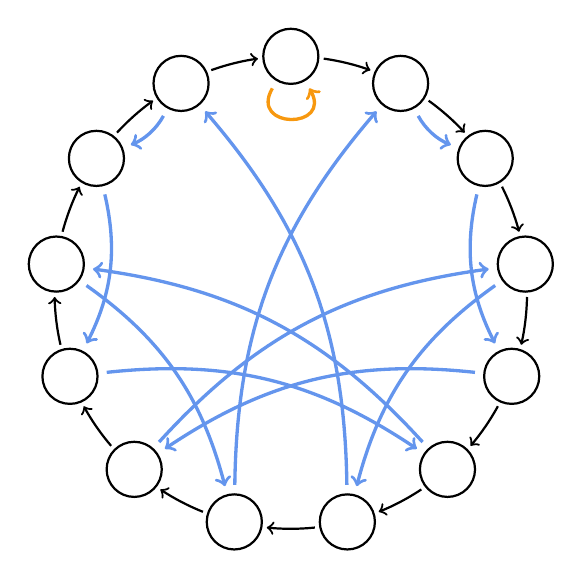
\begin{tikzpicture}[
        thick, every node/.style={circle, draw, minimum size=7mm, inner sep=1pt}]
        \def\n{13}
        \def\mult{2}
        \pgfmathtruncatemacro{\nminusone}{\n-1}
        \def\radius{3cm}
        
        \foreach \i in {0,...,\nminusone} {
          \pgfmathsetmacro{\value}{int(\i)}
          \node (N\i) at ({90-360/\n*(\i)}:\radius) {};
        }
        
        \foreach \i in {0,...,\nminusone} {
          \pgfmathsetmacro{\angle}{90-360/\n*(\i-1)}
          \draw[->] 
          ({\angle-8}:\radius)
          arc[start angle={\angle-8}, delta angle={-360/\n+16}, radius=\radius];
        }
        
        \draw[very thick,YellowOrange,->,shorten >= 3pt,shorten <= 3pt] (N0) to[out=240,in=300,looseness=5] (N0);
        
        \foreach \i in {1,...,\nminusone} {
          \pgfmathtruncatemacro{\j}{mod(\mult*\i,\n)}
          \pgfmathtruncatemacro{\d}{mod(\j-\i+\n,\n)}
          \pgfmathtruncatemacro{\useRight}{(\d <= \n/2 ? 1 : 0)}
          \ifnum\useRight=1
            \draw[very thick, CornflowerBlue, ->, shorten >= 3pt, shorten <= 3pt]
            (N\i) to[bend right=20] (N\j);
          \else
            \draw[very thick, CornflowerBlue, ->, shorten >= 3pt, shorten <= 3pt]
            (N\i) to[bend left=20] (N\j);
          \fi
        }
      \end{tikzpicture}  
    \end{center}
    \vspace*{\stretch{.5}}
    {\superhuge \textbf{\VolumeTitle}\par}
    \vspace*{\stretch{1}}
    {\Large Book II of\par}
    \vspace*{\stretch{.5}}
    {\huge \textsc{\SeriesTitle}\par}
    \vspace*{\stretch{2}}
    {\Large\Version{0}}
  \end{center}
\end{titlepage}
